\subsection{Throttle Communications}\label{sec:eval_rate_limiting}

In the subsequent analysis, we investigate the implications of throttling FSDP communications. As expounded in Section~\ref{sec:memory_management}, launching \code{AllGather} too aggressively can lead to unnecessarily high memory footprint, as the CPU thread needs to allocate CUDA memory blocks when the communication kernel is added into the CUDA stream. This predicament may sometimes result in significant performance problems when the CPU thread runs too fast in comparison to CUDA streams. To gauge its efficacy in varying scenarios, we apply rate limiting to three different types of models and applied the maximum feasible batch size in each experiment.

\begin{itemize}
    \item \textbf{RegNet}~\cite{schneider2017regnet}: model size 9B, and batch size 48 for 2 nodes and 72 for 4 nodes.
    \item \textbf{T5}~\cite{raffel2020exploring}: model size 11B, and batch size 2. 
    \item \textbf{DeepViT}~\cite{zhou2021deepvit}: model size 8B, and batch size 105 for 2 nodes and 120 for 4 nodes. 
\end{itemize}


%\begin{figure}
%    \centering
%    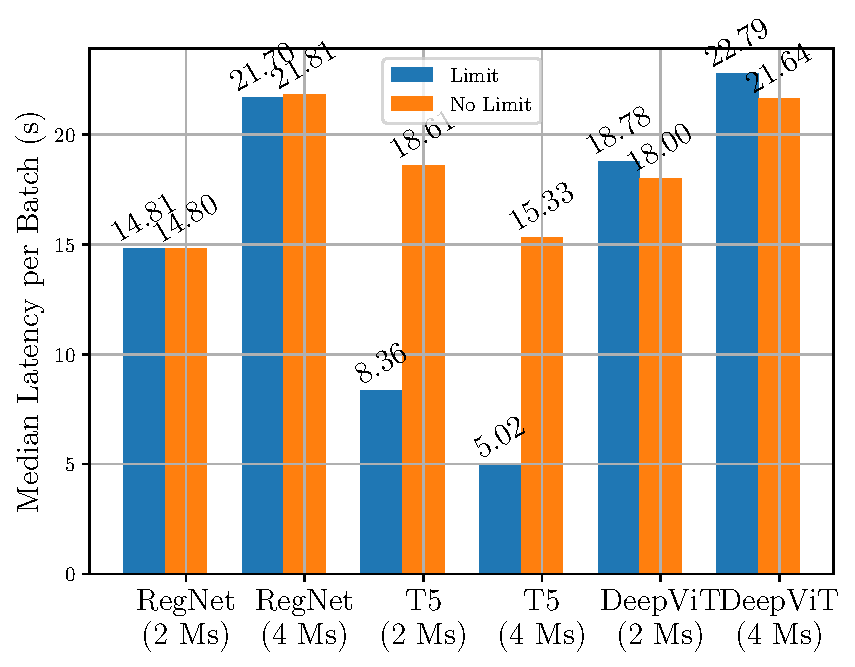
\includegraphics[width=\linewidth]{figure/rate_limiter_latency.pdf}
%    \caption{Rate Limiter On/Off: with 40GB A100, 8 GPUs per Machine %    \label{fig:rate_limiter_latency}
%\end{figure}

Experiment results are plotted in Figure~\ref{fig:mix}~(c).  One notable observation is that the rate limiter's effectiveness is not consistent, as it does not attain any speedups in the RegNet experiments, and even impedes the DeepViT ones. This behavior is expected since throttling the communications can only boost training if the fast CPU thread aggressively allocates GPU memory blocks and causes defragmentations. If it is difficult to identify with certainty from latency measurements or profiled traces, CUDA \code{malloc} retry can serve as a helpful indicator, which can be obtained from the \code{num\_alloc\_retries} key in the \code{torch.cuda.memory\_stats()} dictionary.

The experiments conducted with T5 models have demonstrated that the rate limiter technique can greatly benefit training efficiency, yielding up to 5X speedups. However, for DeepViT models, introducing communication throttling can result in an additional 5\% overhead. This is due to the fact that delaying the \code{AllGather} communication can potentially block subsequent model computations that rely on the \code{AllGather}ed parameters, especially in cases where communication is the dominant factor. Therefore, before enabling rate limiting, practioners should verify whether defragmentation has taken place during training.  

